\documentclass[11pt]{article}

% ---- packages (Overleaf-safe, no exotic deps) ----
\usepackage[utf8]{inputenc}
\usepackage[T1]{fontenc}
\usepackage{lmodern}
\usepackage[margin=1in]{geometry}
\usepackage{amsmath,amssymb}
\usepackage{graphicx}
\usepackage{booktabs}
\usepackage{authblk}
\usepackage{xcolor}
\usepackage{hyperref}
\hypersetup{colorlinks=true,linkcolor=blue,citecolor=blue,urlcolor=blue}
\usepackage{caption}

\newcommand{\todo}[1]{\textcolor{red}{\textbf{[#1]}}}
\newcommand{\pending}{\textcolor{red}{\emph{(pending sweep)}}}

\title{\textbf{A reproducible tissue-damage benchmark for serial-section\\
spatial-transcriptomics registration}}

\author[1]{Rushil Maniar}
\author[1]{Sean Lee}
\author[2]{Sunyoung Lee, MD}
\affil[1]{Sutura Genomics \quad \texttt{\{rushil,sean\}@suturagenomics.bio}}
\affil[2]{Department of \todo{dept}, MD Anderson Cancer Center \quad \texttt{sslee1@mdanderson.org}}
\date{\today}

\begin{document}
\maketitle

\begin{abstract}
Serial-section spatial transcriptomics requires registering consecutive tissue
sections into a common coordinate frame. In practice those sections are
\emph{damaged}---torn on the slide, folded, cut, or partially lost---yet
registration methods are almost always benchmarked on clean tissue, and their
behaviour as damage increases is uncharacterised. We introduce (i) a
reproducible, seeded generator of four physically-motivated damage types
(tear, tissue loss, fold, stretch) with exact per-spot ground-truth transforms;
(ii) a harness that sweeps damage severity against every available registration
method; and (iii) a degradation leaderboard on the spatialLIBD DLPFC corpus,
whose Visium array coordinates provide spot-level ground-truth correspondence
invariant to the applied damage. All experiments are CPU-only and use public
data with no gated models or downloaded weights. We report where each method
breaks, at what severity, and whether its compute cost is justified by
damage robustness. \pending{} for the quantitative leaderboard.
\end{abstract}

\section{Introduction}
Spatial transcriptomics platforms such as 10x Visium profile gene expression at
thousands of spatially-barcoded spots per tissue section. Building a
three-dimensional or multi-section view requires \emph{registration}: mapping
each spot of a moving section into the coordinate frame of a reference section
\cite{zeira2022paste}. Registration quality is the load-bearing step for every
downstream 3D analysis.

Real serial sections are rarely pristine. Cryosectioning and slide handling tear
tissue, fold flaps over, cut through regions, and lose material at the margins.
These are not smooth deformations---tears and folds change the local topology of
the section---and they are precisely the regime in which smooth-deformation
registration assumptions are expected to fail. Yet published benchmarks evaluate
registration on clean or lightly-perturbed tissue, and no systematic
characterisation exists of \emph{how registration accuracy degrades as tissue
damage increases}. This paper provides that characterisation.

\paragraph{Contributions.}
\begin{enumerate}
  \item \textbf{A damage generator} (\S\ref{sec:damage}): a standalone,
  pip-installable, seeded package producing four damage types over five severity
  levels, each emitting a damage mask and an \emph{exact} per-spot ground-truth
  displacement, so registration error is measurable to the spot.
  \item \textbf{A degradation harness} (\S\ref{sec:harness}): a resumable,
  incremental sweep of every installable registration method across the full
  damage grid, with honest reporting of methods that do not install.
  \item \textbf{A leaderboard} (\S\ref{sec:results}): degradation curves,
  failure rates, and compute cost on the spatialLIBD DLPFC serial-section corpus.
  \item \textbf{Common-spot scoring} (\S\ref{sec:abstention}): we show that
  partial-registration methods can \emph{abstain}---decline to place spots---and
  that scoring only matched spots systematically flatters them; we give a worked
  case where this reverses a headline result, and prescribe a scoring protocol
  that closes the loophole.
\end{enumerate}

\paragraph{Scope.} We deliberately exclude single-cell foundation-model
featurizers. Their zero-shot representations already underperform simple
baselines on spatial clustering and integration \cite{kedzierska2023assessing},
and in our environment none of five candidate models (scGPT
\cite{cui2024scgpt}, Geneformer \cite{theodoris2023geneformer}, UCE,
scFoundation, Nicheformer) installs and imports on CPU
(Appendix~\ref{sec:envcheck}). The question here is not representation learning
but \emph{registration robustness under damage}, evaluated on classical methods.

\section{The damage model}
\label{sec:damage}
Let a section be a set of spot coordinates $X=\{x_i\}_{i=1}^{n}\subset\mathbb{R}^2$
with median nearest-neighbour pitch $p$ (all magnitudes are expressed in units of
$p$ so they transfer across sections). A damage operator
$\mathcal{D}_{t,\ell,s}$ is parameterised by type $t$, integer severity level
$\ell\in\{0,\dots,5\}$ (with $\ell{=}0$ the undamaged control), and seed $s$. It
returns, for each surviving spot, a damaged coordinate and the exact forward
displacement $d_i = \tilde{x}_i - x_i$; removed spots are flagged in a mask.
Registration ground truth is $\mathcal{D}^{-1}$: a method that recovers the
original coordinate scores zero error. $\mathcal{D}_{t,\ell,s}$ is a pure
function of $(t,\ell,s)$---the same triple reproduces the section bit-for-bit.

\paragraph{Tear.} A cut propagating along a path---not a random blob. We generate
a path crossing the section with three geometries: \emph{straight} (a chord),
\emph{curved} (a sinusoidal wander about the chord), and \emph{branching} (a main
path plus one fork). Spots within a narrow blade half-width of the path are
removed; the remaining spots on each side retract along the \emph{local} cut
normal by half the tear gap, so the two lips separate perpendicular to the cut
everywhere along the path. The gap (in pitches) sets severity. The result is a
piecewise-rigid, topology-changing displacement---the canonical failure case for
smooth-deformation registration.

\paragraph{Tissue loss.} A contiguous, edge-anchored region is removed. A seed is
chosen at a section boundary and the nearest spots under an angularly-modulated
metric are excised, giving an organic (non-circular) boundary. Severity is the
fraction of spots removed (5--50\%). Surviving spots are undisplaced; the
challenge is partial overlap, the regime partial-optimal-transport methods
(PASTE2 \cite{liu2023paste2}) target.

\paragraph{Fold.} A flap is doubled over a fold line: spots beyond the line are
reflected across it and overlap the body, creating a region of doubled spot
density. Severity is the folded flap's fraction of the section extent. The
reflection is an exact, invertible map that no globally-smooth deformation can
represent.

\paragraph{Stretch.} A local non-rigid deformation near a boundary: a
Gaussian-weighted radial expansion about a boundary anchor, with peak
displacement (in pitches) setting severity. Unlike tear/fold it is continuous,
isolating smooth-deformation error from topology change.

\begin{figure}[t]
  \centering
  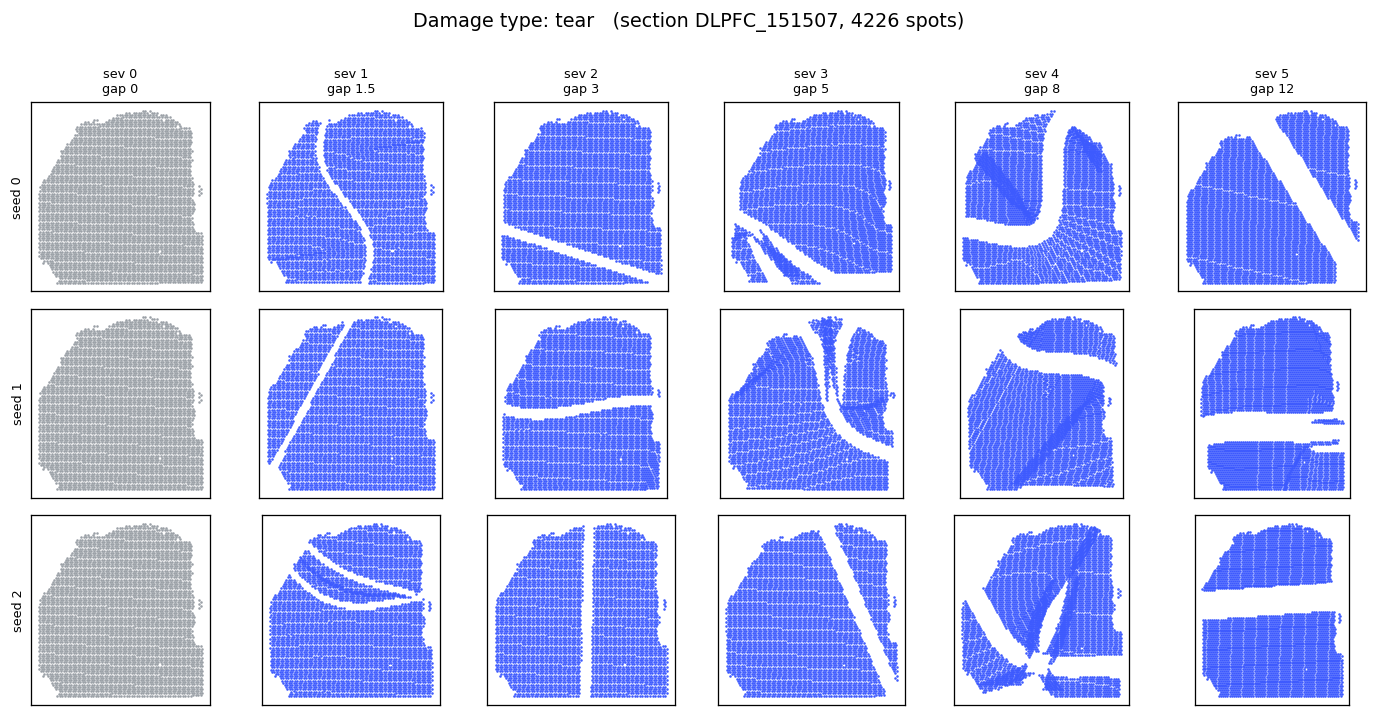
\includegraphics[width=\linewidth]{../results/damage_examples/tear_grid.png}
  \caption{Tear damage on DLPFC section 151507 across severity (columns, gap in
  spot-pitches) and seed (rows). Severity 0 is the undamaged control. Grey =
  intact, red = removed (blade path), blue = displaced. Seeds sample the three
  tear geometries.}
  \label{fig:tear}
\end{figure}

\begin{figure}[t]
  \centering
  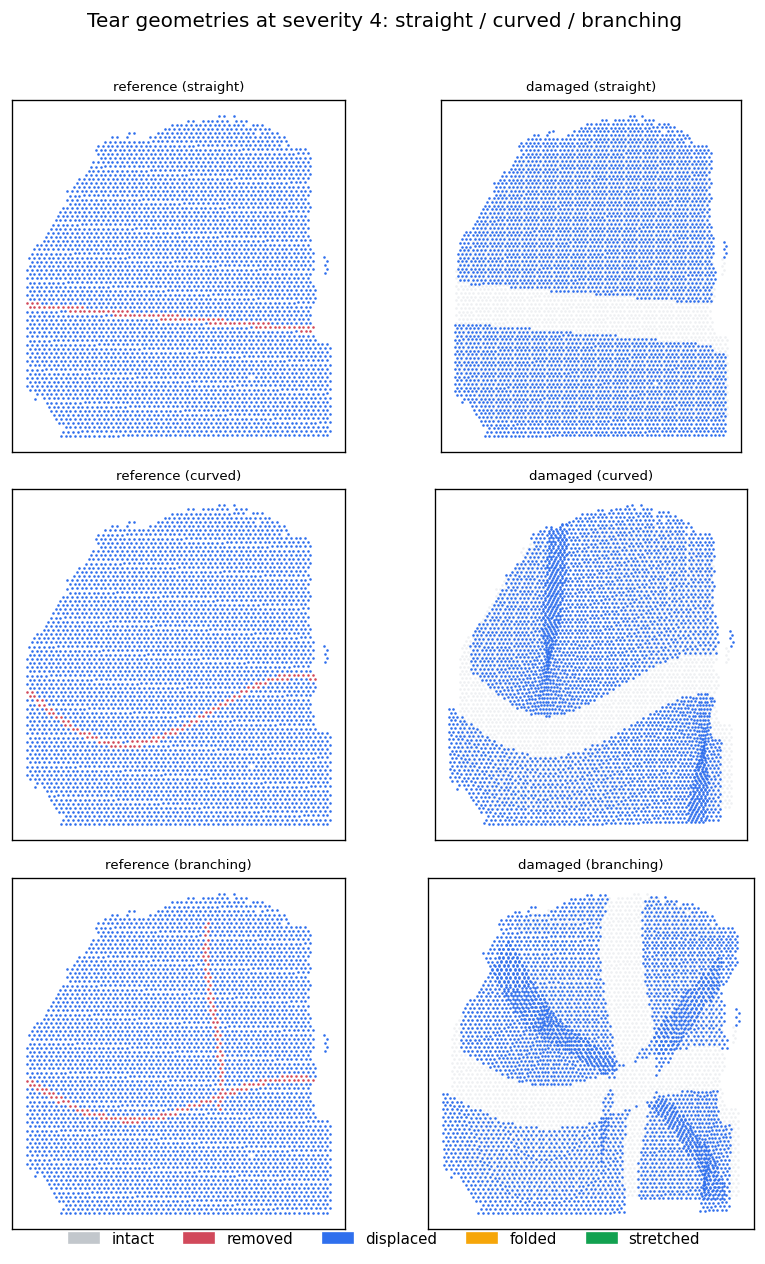
\includegraphics[width=\linewidth]{../results/damage_examples/tear_geometries.png}
  \caption{Tear path geometries at severity 4: straight, curved, branching.}
  \label{fig:teargeo}
\end{figure}

\begin{figure}[t]
  \centering
  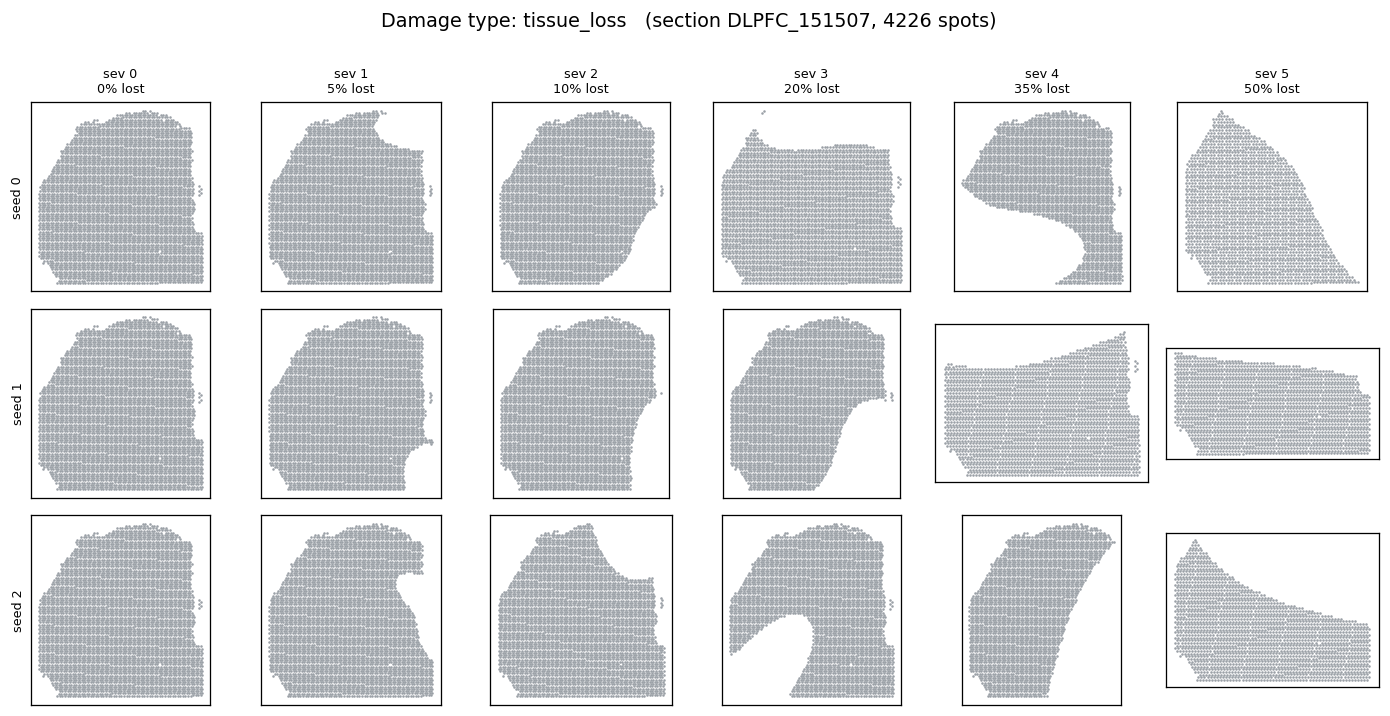
\includegraphics[width=0.49\linewidth]{../results/damage_examples/tissue_loss_grid.png}
  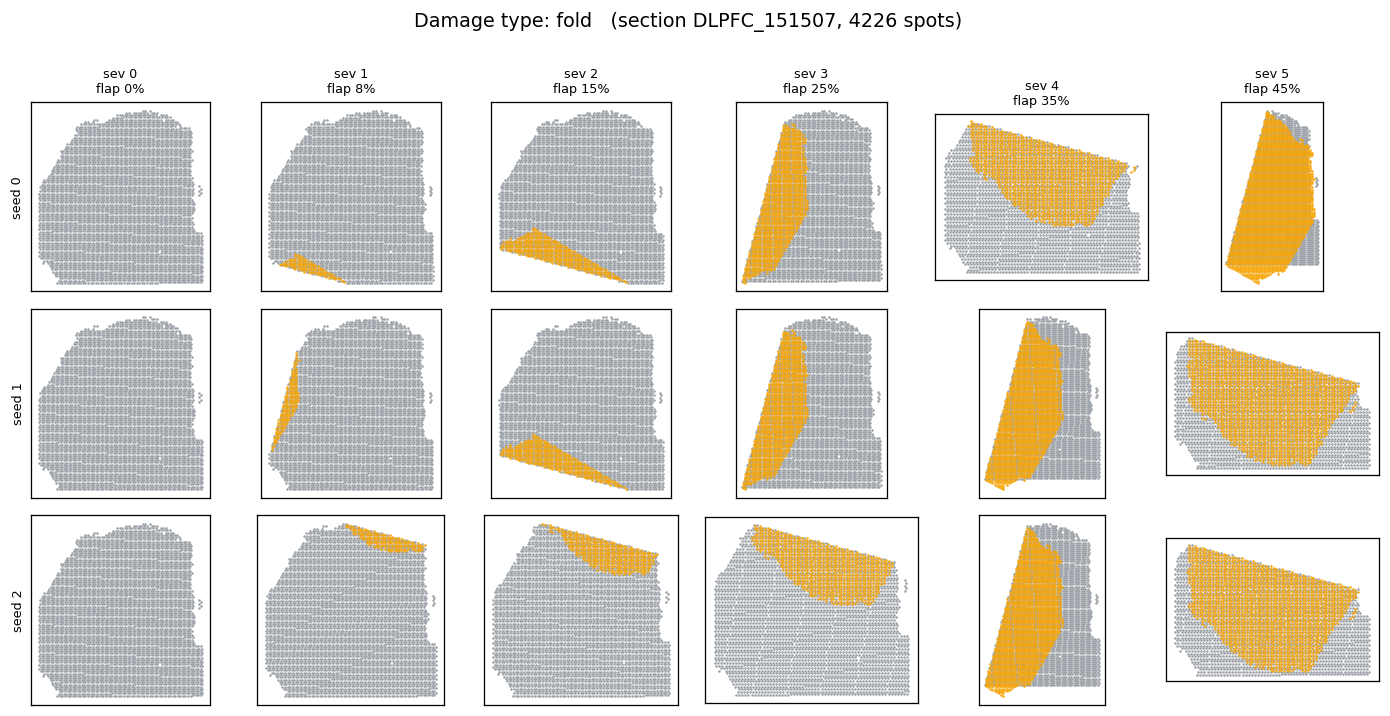
\includegraphics[width=0.49\linewidth]{../results/damage_examples/fold_grid.png}\\
  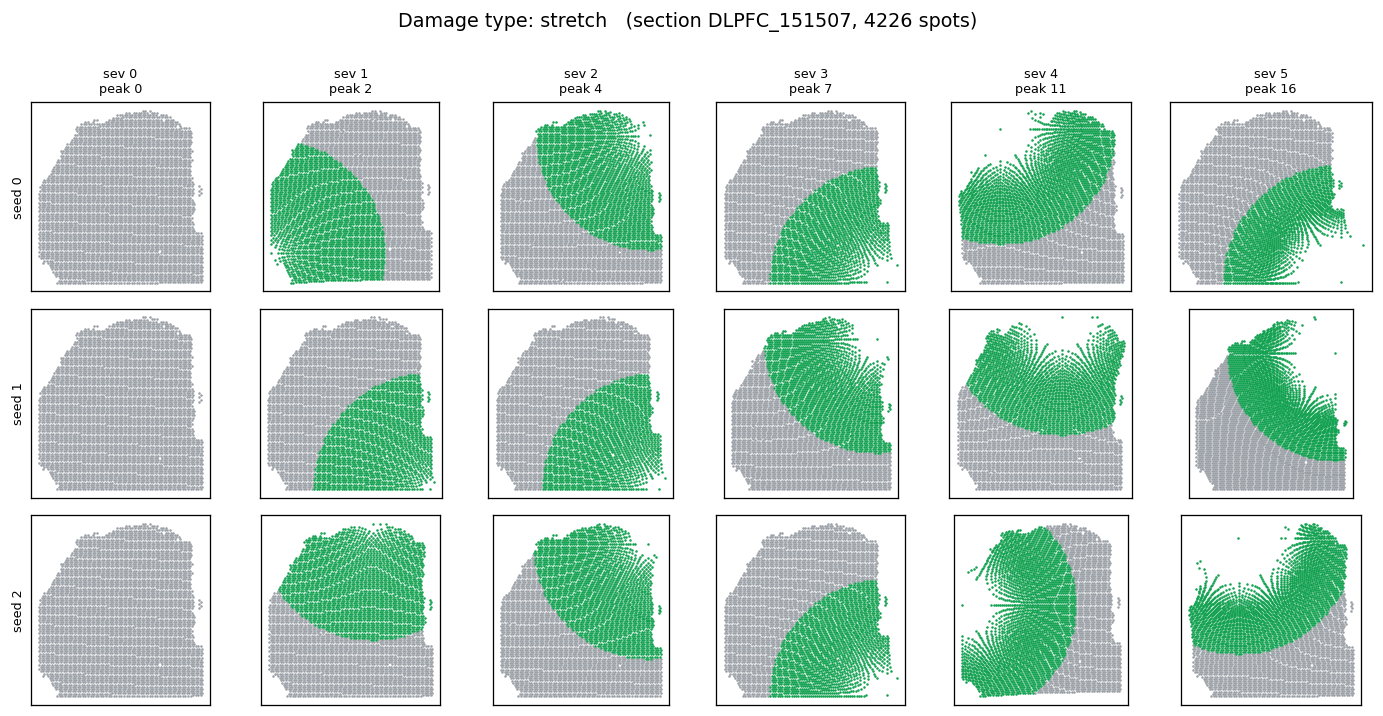
\includegraphics[width=0.49\linewidth]{../results/damage_examples/stretch_grid.png}
  \caption{Tissue loss (organic edge-anchored removal, 5--50\%), fold (orange
  flap doubled over the body), and stretch (green local radial deformation),
  across severity and seed.}
  \label{fig:others}
\end{figure}

\section{Corpus and ground truth}
We use the spatialLIBD dorsolateral prefrontal cortex (DLPFC) dataset
\cite{maynard2021transcriptome}: 12 Visium sections from 3 donors
($\times$ 4 consecutive sections). Adjacent within-donor sections are serial
pairs. The Visium array index $(\text{row},\text{col})$ is preserved under our
coordinate-space damage, giving a spot-level correspondence between reference and
moving section that is invariant to the applied transform---the registration
ground truth. This is the entire corpus by design; no other datasets are added.
DLPFC additionally carries manual seven-class cortical-layer annotations
(Layer 1--6 + white matter), enabling a label-transfer metric.

\section{Methods under test}
\label{sec:methods}
\begin{itemize}
  \item \textbf{rigid} --- a parameter-free similarity transform (rotation,
  isotropic scale, translation) fit from the two point clouds' moments alone, no
  expression. The floor a useful method must beat; it cannot represent tears or
  folds.
  \item \textbf{PASTE} \cite{zeira2022paste} --- Fused Gromov--Wasserstein optimal
  transport on expression + spatial structure.
  \item \textbf{PASTE2} \cite{liu2023paste2} --- partial OT, designed for partial
  overlap (our tissue-loss regime).
  \item \textbf{STalign} \cite{clifton2023stalign} --- LDDMM diffeomorphic image
  registration.
  \item \textbf{GPSA} \cite{jones2023gpsa} --- Gaussian-process spatial alignment.
\end{itemize}
Each method is probed for real installability; those that do not install in a
given environment are recorded with their exact error and skipped, never stubbed
with a fabricated API (Appendix~\ref{sec:methodenv}).

\section{Harness and metrics}
\label{sec:harness}
For every serial pair, damage type, severity, and seed, the moving section is
damaged and registered to the reference by each available method. Sections are
subsampled to a fixed spot budget ($\sim$2000 spots) so partial-OT methods are
CPU-tractable.

\paragraph{Common-spot scoring.} Registration error is the per-spot displacement
between a method's predicted coordinate and the array-bridge ground truth, in
pitches. Every method is scored on the \emph{same} set of spots: the common
ground-truth-matchable set for that cell (all moving spots with a known reference
correspondence). A method that declines to place a spot---a partial-OT plan can
leave a spot with essentially zero transported mass---does not have that spot
dropped from its error; the unmatched spot is penalised with the error of the
best uninformed predictor (the reference-tissue centroid). This removes the
abstention bias analysed in \S\ref{sec:abstention}. For every cell we record, as
first-class columns, the number of spots scored (\texttt{n\_scored}), the
fraction a method left unmatched (\texttt{unmatched\_frac}), and, for partial-OT,
the overlap parameter $s$ used; PASTE2 is reported at both its heuristic
$s{=}n_\text{mov}/n_\text{ref}$ and at $s{=}1$ (no abstention), so its
parameterisation is fully visible to the reader.

We further record mean displacement, cortical-layer label-transfer accuracy,
runtime, and failure rate (crashes plus degenerate/collapsed transforms). The
harness is single-instance-locked, resumable (skips completed cells), writes a
per-cell heartbeat, and writes one CSV row per
$(\text{donor}\times\text{pair}\times\text{type}\times\text{severity}\times
\text{seed}\times\text{method}\times\text{metric})$ incrementally.

\section{Abstention bias in partial-registration benchmarks}
\label{sec:abstention}
Partial-registration methods can \emph{abstain}: a partial-optimal-transport plan
(PASTE2) with overlap parameter $s<1$ transports only an $s$-fraction of the mass
and can leave individual moving spots with essentially zero coupling, hence no
predicted location. A benchmark that averages error only over matched spots
therefore grades such a method on the subset of spots it chose to answer---
systematically flattering it, and worst exactly in the partial-overlap regime
these methods target.

We encountered this directly. Our adapter set PASTE2's overlap to the observed
spot ratio $s=n_\text{mov}/n_\text{ref}$. On a 50\%-tissue-loss section of DLPFC
pair 151507/151508 this gives $s=0.5$, and PASTE2 leaves $\approx$43\% of the
surviving moving spots unmatched. Scored only on the $\approx$250 spots it did
match, its median error ($\approx$6 pitches) looks competitive with the
parameter-free rigid floor---which is scored on all $\approx$410 matchable spots.
The comparison is not apples-to-apples. Forcing $s{=}1$ removes the abstention,
PASTE2 now places all $\approx$430 spots, and its median error rises to
$\approx$12 pitches: the abstention was \emph{concealing} the loss, not causing
it. The honest, common-spot result is that partial OT loses to the rigid floor
on heavy tissue loss by roughly $2\times$---in the very regime it was built for.

We therefore adopt \textbf{common-spot scoring} (\S\ref{sec:harness}) as a
benchmark requirement whenever any method can abstain: (i) score every method on
the same common ground-truth-matchable spot set; (ii) penalise unmatched
predictions rather than dropping them; (iii) report \texttt{n\_scored},
\texttt{unmatched\_frac}, and the partial-overlap parameter for every cell; and
(iv) report partial methods at both their heuristic and their no-abstention
parameterisation. Without these, a partial method's headline accuracy is partly a
function of how much it declined to answer. We flag this as a reusable pitfall for
spatial-registration benchmarks, not a quirk of one tool.

\section{Results}
\label{sec:results}
\pending{} All numbers await the common-spot re-run (\S\ref{sec:abstention}); no
provisional or abstention-biased numbers are reported here. On completion this
section reports, under common-spot scoring:
\begin{itemize}
  \item Degradation curves (median error vs severity, one line per method,
  faceted by damage type): \texttt{results/degradation\_curves.png}.
  \item Failure rates by method and damage type:
  \texttt{results/failure\_rates.png}.
  \item Compute cost vs severity: \texttt{results/runtime\_scatter.png}.
  \item A leaderboard of the severity at which each method crosses 1, 2, and 5
  spot-pitch error and where it breaks (failure rate $>50\%$).
\end{itemize}

\begin{table}[h]
  \centering
  \caption{Severity at which each method breaks, per damage type. \pending}
  \label{tab:leaderboard}
  \begin{tabular}{lcccc}
    \toprule
    method & tear & tissue loss & fold & stretch \\
    \midrule
    rigid (floor) & \todo{--} & \todo{--} & \todo{--} & \todo{--} \\
    PASTE  & \todo{--} & \todo{--} & \todo{--} & \todo{--} \\
    PASTE2 & \todo{--} & \todo{--} & \todo{--} & \todo{--} \\
    GPSA   & \todo{--} & \todo{--} & \todo{--} & \todo{--} \\
    STalign & \todo{--} & \todo{--} & \todo{--} & \todo{--} \\
    \bottomrule
  \end{tabular}
\end{table}

\section{Discussion}
\pending{} for all quantitative claims; the structural argument below does not
depend on the numbers.

\paragraph{Diffeomorphic registration cannot represent a tear.} STalign---like
CODA and other LDDMM methods---computes a diffeomorphism: a smooth, invertible map
with a smooth inverse. A diffeomorphism preserves topology by construction; it
cannot tear, merge, or otherwise change the connectivity of its domain. A physical
tear is precisely a change of topology---a connected region separates---so no
diffeomorphism can represent it, at any smoothness scale or iteration count.
STalign's large error on torn tissue (\pending{} pitches) is therefore not a
tuning failure to be closed with better hyperparameters; it is a structural
impossibility of the diffeomorphic model class---the failure lives in the
hypothesis space, not the optimiser. This is the paper's central argument for why
torn serial sections need a registration model that is not constrained to be
diffeomorphic.

All remaining claims await the common-spot sweep (\S\ref{sec:abstention}): whether
topology-changing damage (tear, fold) degrades smooth-deformation methods faster
than tissue loss; whether partial-OT PASTE2 escapes the rigid floor in the
tissue-loss regime it targets; whether any method meaningfully beats the rigid
floor at high severity; and whether heavier methods (GPSA) earn their compute.
Negatives are reported plainly.

\section{Limitations}
\label{sec:limitations}
\textbf{Interior damage vs.\ boundary-reaching tears.} For the four primary
damage types the section's outer boundary remains a closed polygon while damage
opens internally---the tear is a crack in a fixed plate, not a separation that
reaches the tissue edge. Real torn sections have lips that separate at the
boundary, opening the outline itself. Our primary damage therefore makes the task
\emph{easier than reality}: a registration method can anchor on the intact
outline. We accept this because exact per-spot ground truth is worth more than
visual realism here; we do not hide it. A secondary boundary-reaching tear
(\texttt{tear\_edge}, Fig.~\ref{fig:teargeo}), whose slit opens the outline, is
included at severity $\{0,4\}$ to probe this gap, but the primary leaderboard is
on interior damage. \textbf{Self-damage plus synthetic misalignment.} The moving
section is a damaged copy of itself under a known rigid misalignment, not a
biologically distinct serial section; this isolates the damage effect but omits
real inter-section variation. \textbf{Methods included.} STalign installs only on
Python 3.11 + numpy$<$2; wired to its real LDDMM API it runs on every damage type
and is included (it is slow on CPU). PASTE's internal fused-Gromov--Wasserstein
breaks against POT$\geq$0.9's \texttt{line\_search}, which added a positional
gradient argument its closures reject; we patch it with a scoped compatibility
shim, so both PASTE and its partial-OT successor PASTE2 are included. All five
methods run under one environment.

\section{Reproducibility}
The damage generator is a standalone package (\texttt{pip install -e damage});
every damaged section is reproducible from $(\text{type},\text{severity},
\text{seed})$. Code, the damage renders, the environment audits, and (on
completion) the results CSV and figures are in the repository.

\appendix
\section{Foundation-model environment audit}
\label{sec:envcheck}
\pending{table from \texttt{results/env\_check.md}} All five candidate single-cell
foundation models are unusable on the target host (Windows, CPU, Python 3.14):
scGPT and Geneformer install but fail to import; UCE, scFoundation, and
Nicheformer do not install. Exact errors are logged.

\section{Registration-method environment audit}
\label{sec:methodenv}
\pending{table from \texttt{results/methods\_env.md}} \texttt{rigid}, PASTE, and
PASTE2 are available; STalign fails to build its pinned NumPy on Python 3.14;
GPSA requires a local install.

\bibliographystyle{plain}
\bibliography{refs}

\end{document}
